\documentclass{article}

% if you need to pass options to natbib, use, e.g.:
%     \PassOptionsToPackage{numbers, compress}{natbib}
% before loading neurips_2018

% ready for submission
% \usepackage{neurips_2018}

% to compile a preprint version, e.g., for submission to arXiv, add add the
% [preprint] option:
%     \usepackage[preprint]{neurips_2018}

% to compile a camera-ready version, add the [final] option, e.g.:
%     \usepackage[final]{neurips_2018}

% to avoid loading the natbib package, add option nonatbib:
%     \usepackage[nonatbib]{neurips_2018}

\usepackage[utf8]{inputenc} % allow utf-8 input
\usepackage[T1]{fontenc}    % use 8-bit T1 fonts
\usepackage{hyperref}       % hyperlinks
\usepackage{url}            % simple URL typesetting
\usepackage{booktabs}       % professional-quality tables
\usepackage{amsfonts}       % blackboard math symbols
\usepackage{nicefrac}       % compact symbols for 1/2, etc.
\usepackage{microtype}      % microtypography
\usepackage{graphicx}
\usepackage{amsmath}
\usepackage{amssymb}

\title{Applying Image Inpainting to Video Post Production}

% The \author macro works with any number of authors. There are two commands
% used to separate the names and addresses of multiple authors: \And and \AND.
%
% Using \And between authors leaves it to LaTeX to determine where to break the
% lines. Using \AND forces a line break at that point. So, if LaTeX puts 3 of 4
% authors names on the first line, and the last on the second line, try using
% \AND instead of \And before the third author name.

\author{%
  Bryce Haley \\
  \texttt{bhaley@sfu.ca} \\
  % examples of more authors
  \and
  Di Wang \\
  % Affiliation \\
  % Address \\
  \texttt{dwa92@sfu.ca} \\
  \and
  Hyukho Kwon \\
  % Affiliation \\
  % Address \\
  \texttt{hyukhok@sfu.ca} \\
  \and
  Joshil Patel \\
  % Affiliation \\
  % Address \\
  \texttt{joshilp@sfu.ca} \\
  \and
  Kino Roy \\
  % Affiliation \\
  % Address \\
  \texttt{kroy@sfu.ca} \\
}

\begin{document}
% \nipsfinalcopy is no longer used

\maketitle

\begin{abstract}
  
  This paper attempts to apply existing U-net Architecture presented in an earlier NVIDIA's paper[1] for image in-painting to videos without recruiting the use of a time sensitive models such as an LSTM. The network was trained on  $512\times512$ images from the ImageNet set. Then tested on publicly available video in 720p. Strong results were achieved when infilling some noisy backgrounds such as ocean waves but displayed flickering and other artifacts when trying to reproduce more structured backgrounds. 
\end{abstract}

\section{Motivation}

\paragraph{}
In the Visual Effects (VFX) industry, \textit{inpainting} is a process where artists remove unwanted objects or artifacts in a film clip. Often, inpainting is done by creating a mask and stenciling each image frame, then painting in the resulting hole. Large sequences can be labour intensive and tedious, thus creating a bottlneck in the VFX pipeline, often slowing down the process for later departments. Using machine learning to automate the inpainting process would therefore, be fruitful in decreasing this bottleneck and could be useful for the VFX industry as a whole.

\section{Approach}
\paragraph{}
\textit{Image Inpainting for Irregular Holes Using Partial Convolutions} (Liu et al. 2018) shows convincing results for predicting masked-out portions of an image [1]. This paper will attempt to extend the work by Liu et al. to apply their image inpainting process to a VFX application.

\subsection{Partial Convolution}
\paragraph{}
Convolutional neural networks have been the standard for image inpainting methods in the past, and have shown excellent performance at extracting high-level features of images. Liu et al. proposes a \textit{partial} convolution network where only masked areas are passed as inputs. This approach appears to outperform previous methods for irregular masks.

Let $\mathbf{W}$ the weights for the convolution filter and $\mathit{b}$ be the corresponding bias. $\mathbf{X}$ are the pixel values for the current convolution window and $\mathbf{M}$ is the corresponding binary mask.
\begin{equation}
	x'=
    \begin{cases}
        \mathbf{W}^{T}(\mathbf{X} \odot \mathbf{M}), & \textrm{if\ sum}(\mathbf{M}) > 0\\
        0, & \text{otherwise}
    \end{cases}
\end{equation}

The mask is updated after each partial convolution. If the convolution was able to condition its output on at least one valid input value, then remove the mask for that location.

\begin{equation}
	m'=
    \begin{cases}
        1, & \textrm{if\ sum}(\mathbf{M}) > 0\\
        0, & \text{otherwise}
    \end{cases}
\end{equation}

The loss function is defined as follows:
\begin{equation}
\mathcal{L}_{\mathrm{total}} = \mathcal{L}_{\mathrm{valid}} + 6 \mathcal{L}_{\mathrm{hole}} + 0.05\mathcal{L}_{\mathrm{perceptual}} + 120( \mathcal{L}_{\mathrm{style_{out}} }+ \mathcal{L}_{\mathrm{style_{comp}}}) +0.1\mathcal{L}_{\mathrm{tv}}
\end{equation}
%$\mathcal{L}_{\mathrm{hole}}$ and $\mathcal{L}_{\mathrm{valid}}$ represent the pixels losses for the hole, and non-hole pixels.
\begin{align*}
    \intertext{where,}
    L_{\mathrm{valid}} &= ||M \odot (I_{\mathrm{out}} - I_{\mathrm{gt}})||_{1}\ (I_{\mathrm{out}} \mathrm{is\ the\ network\ prediction},\ I_\mathrm{gt}\ \mathrm{the\ ground\ truth}) \\
    L_{\mathrm{hole}} &= ||(1-M) \odot (I_{\mathrm{out}} - I_{\mathrm{gt}})|| \ (M\ \mathrm{is\ the\ initial\ binary\ mask})\\
    L_{\mathrm{perceptual}} &= \sum_{n=0}^{N-1} || \psi_n (I_{\mathrm{out}}) -  \psi_n (I_{\mathrm{gt}}) ||_1 + \sum_{n=0}^{N-1} || \psi_n (I_{\mathrm{comp}}) -  \psi_n (I_{\mathrm{gt}}) ||_1\\
    %
    \intertext{Auto-correlation (Gram Matrix) Style Loss:}
    L_{\mathrm{style_{out}}} &= \sum_{n=0}^{N-1} || K_n (( \psi_n (I_{\mathrm{out}}))^T( \psi_n (I_{\mathrm{out}})-(\psi_n (I_{\mathrm{gt}}) )^T(\psi_n (I_{\mathrm{gt}}) )) ||_1\\
    L_{\mathrm{style_{comp}}} &= \sum_{n=0}^{N-1} || K_n (( \psi_n (I_{\mathrm{comp}}))^T( \psi_n (I_{\mathrm{comp}})-(\psi_n (I_{\mathrm{gt}}) )^T(\psi_n (I_{\mathrm{gt}}) )) ||_1
    %
    \intertext{Smoothing Penalty:}
    L_{\mathrm{tv}} &= \sum_{(i,j) \in P,(i,j+1) \in P} || I_{\mathrm{comp}}^{i,j+1}-I_{\mathrm{comp}}^{i,j}||_1+\sum_{(i,j) \in P,(i+1,j) \in P} || I_{\mathrm{comp}}^{i+1,j}-I_{\mathrm{comp}}^{i,j}||_1
\end{align*}

\subsection{U-Net Architecture}

\begin{figure}[ht]
  \centering
  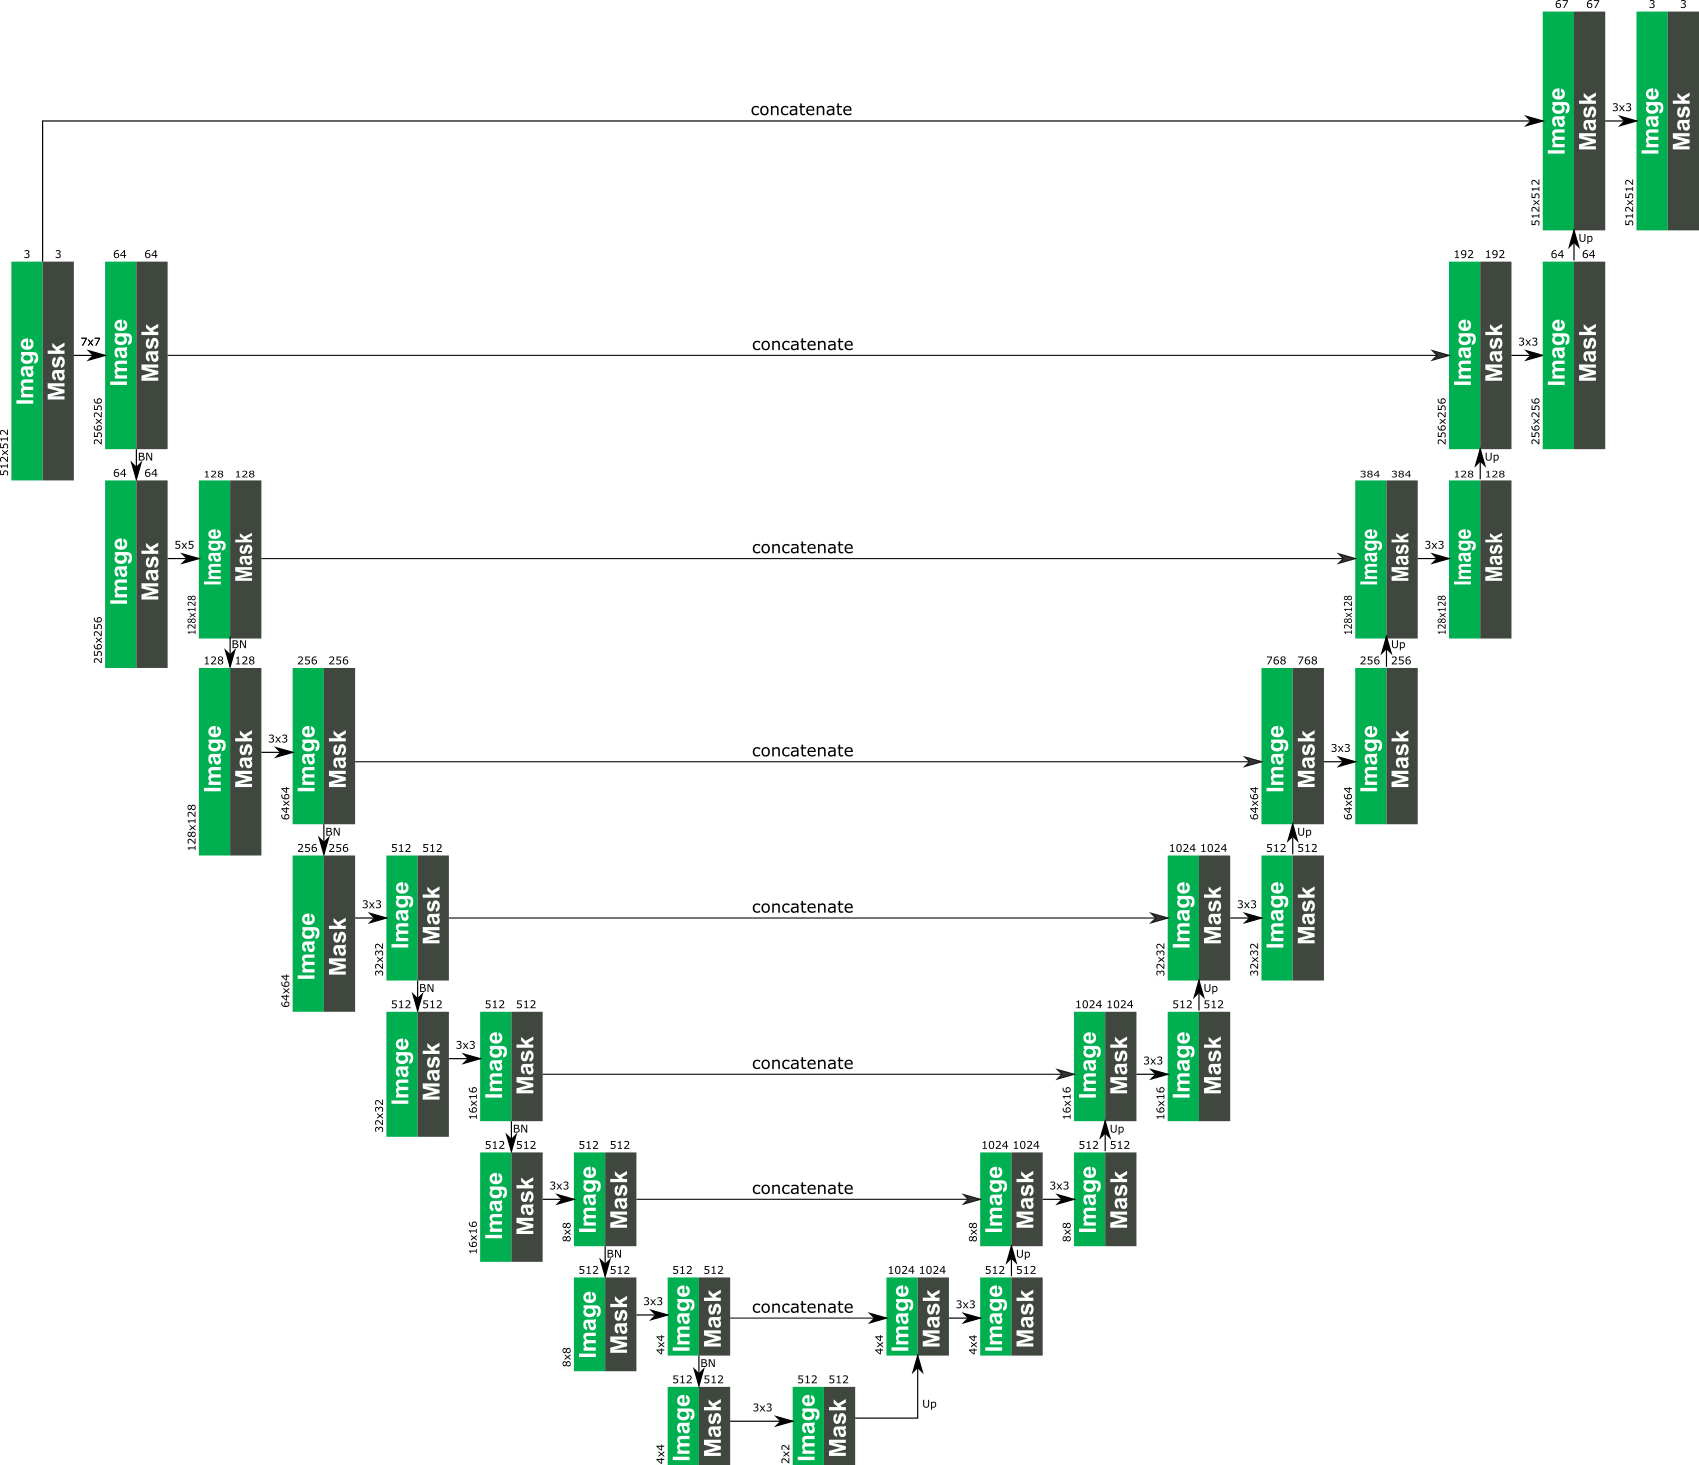
\includegraphics[scale=0.6]{graph.png}
  \caption{U-Net graph}
\end{figure}

\paragraph{}
A U-shaped Network (U-Net) is used to learn image features and to predict pixels in the masked area. The left half of the U-Net is the shrinking stage. The shrinking stage uses down-pooling to aggregate information over large areas of the input images [6]. It is an essential step to learn key features (low-frequency) while putting less weight on details (high-frequency). However, down-pooling results in reduced resolution [6].

\paragraph{}
The right side of the U-Net is the refining stage. It firstly uses up-convolutional layers to extend features by replicating pixels. In order to recover the reduced resolution,  the U-Net “concatenates” the layer with corresponding features from the left layer in each convolution [6]. This then allows the U-Net to predicts the output image which preserves both high-level features passed down from the shrinking state and fine local features provided from the left layers [6]. 



\pagebreak
\section{Data}

\paragraph{}
The ImageNet Large Scale Visual Recognition Challenge (ILSVRC) 2017 dataset was used for training the model [3]. This was also one of the data sets Liu et al. used for training in their original implementation [1].

\paragraph{}
For testing data, seven short video clips were sourced online [3][4]. These clips were then rendered as a sequence of images to be used for the prediction model. Mask data was manually created per clip, and also rendered out as a sequence. 


\section{Code}
\paragraph{}
A Python-based implementation of the NVIDIA paper that uses Keras and TensorFlow, created by Mathias Gruber, can be found on his GitHub repo [2].

\paragraph{}
Gruber implements the the following:

\begin{enumerate}
    \item Creating random irregular masks
    \item Implementing and testing the implementation of the PConv2D layer
    \item Implementing and testing the U-Net architecture with PConv2D layers
    \item Training and testing the final architecture on ImageNet
\end{enumerate}

\paragraph{}
Our work in extending the code base involved modifying it to automate accepting image-sequence pairs representing a frame in a video, coupled with its corresponding mask. The masks we input were manually generated, as opposed to using Gruber's code to generate random masks, as this does not serve our purposes. We then output the frames in an organized way to easily be played as a video frame-by-frame.

\paragraph{}
As the model only accepts images of $512 \times 512$ pixels in size, Gruber implemented convenience functions in his model which, disect an input image into multiple images of the correct size, and then stitch multiple outputs of the model back together into the final prediction for that image. This allowed us to use high resolution videos.


\pagebreak
\section{Results}

\begin{figure}[ht]
  \centering
  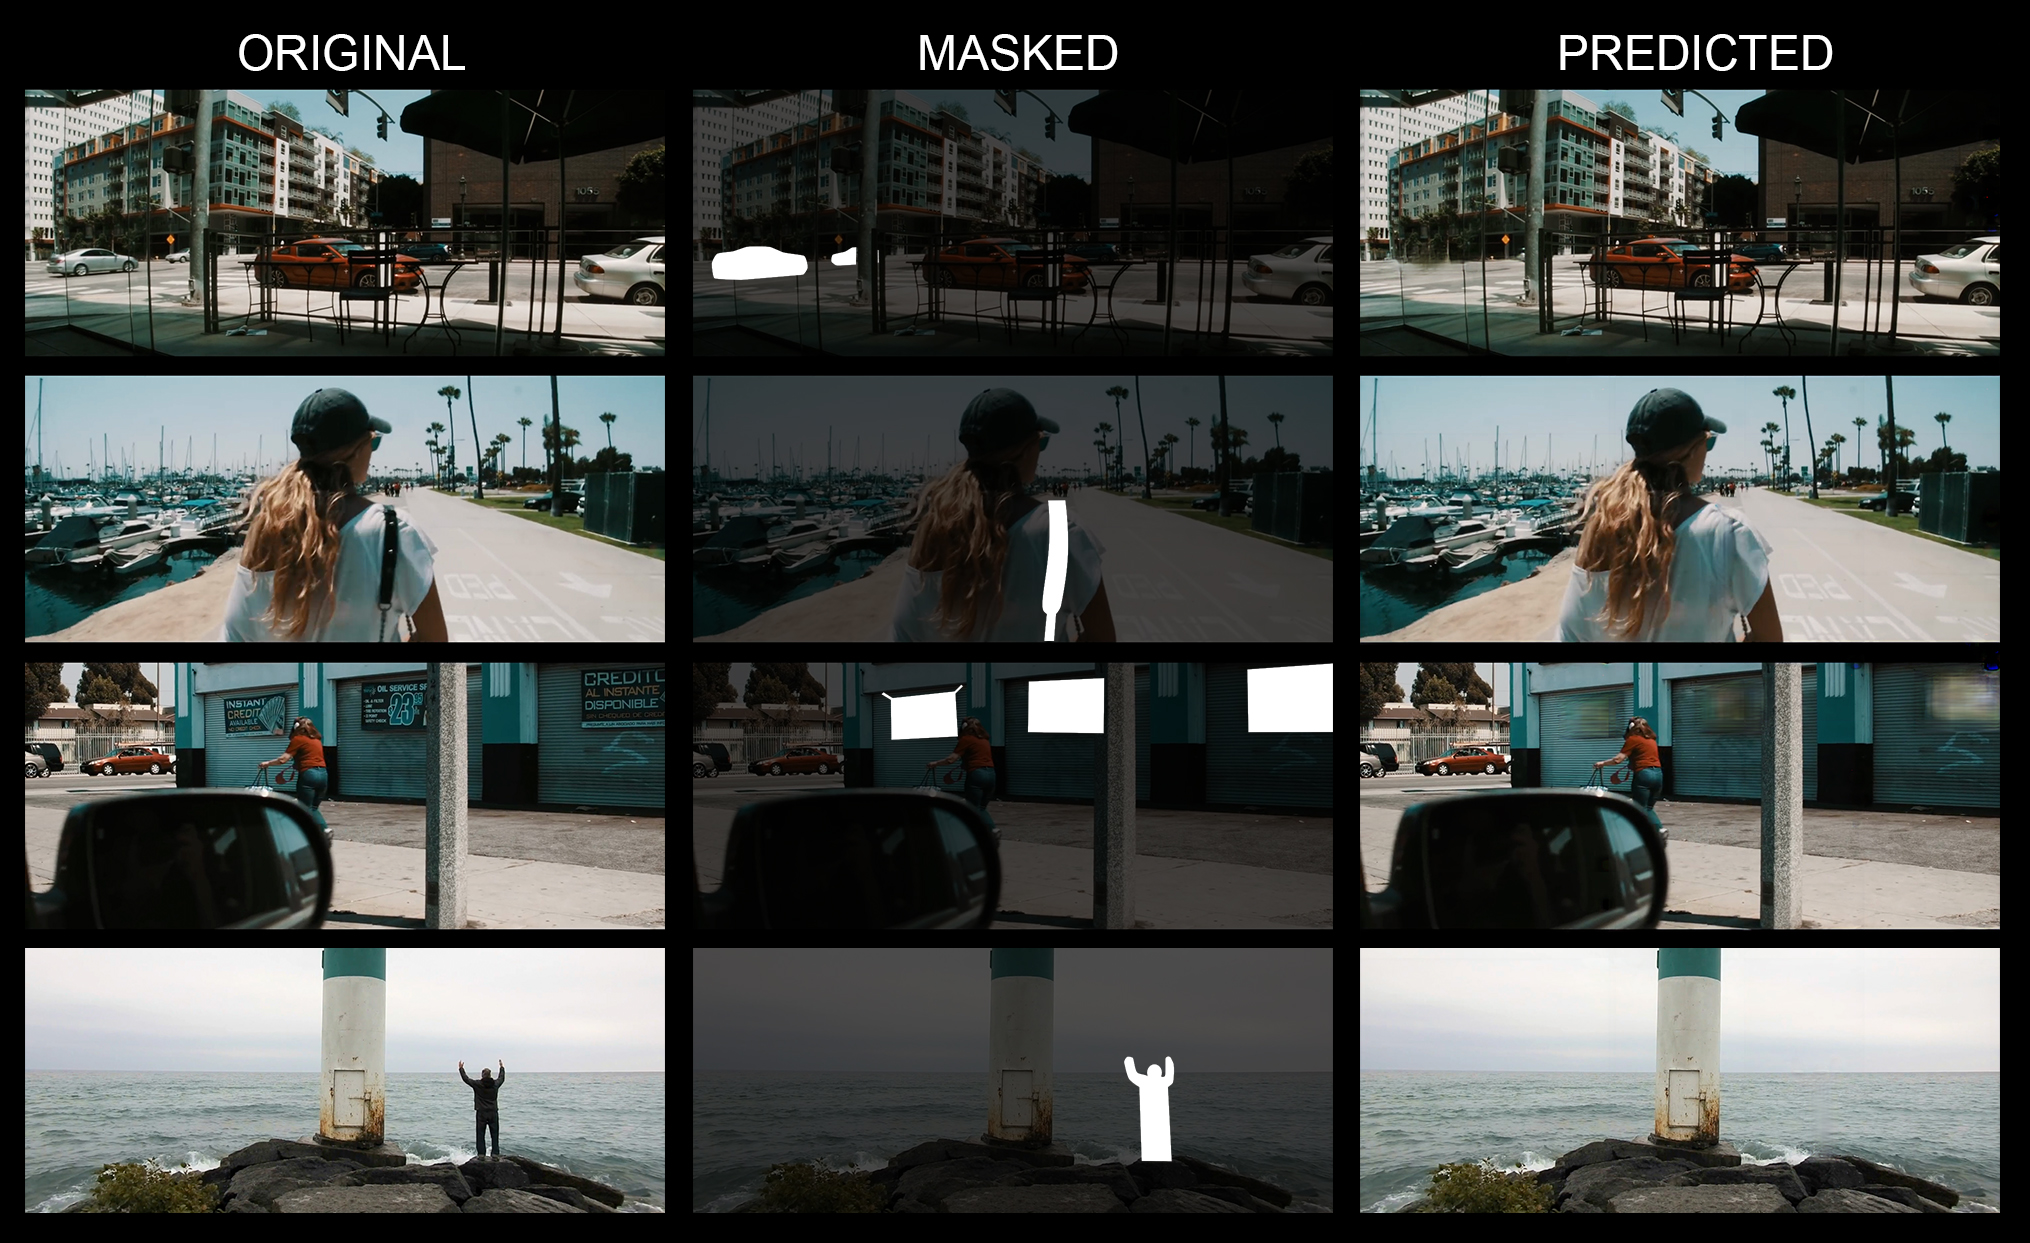
\includegraphics[scale=0.16]{results.jpg}
  \caption{Frames from each of the four test videos comparing ground-truth, masked input, and model prediction.}
\end{figure}

\paragraph{}
Figure 2 displays the prediction results on four chosen sample videos. In order of the images from top to bottom, the objects items removed were two background vehicles in row 1, the bag strap in row 2, the three signs in row 3, and the standing person in row 4.


\subsection{Successes}
\paragraph{}
On a per-frame basis, the prediction model managed to recreate missing masked areas. Row 2 and 4 produced convincing predictions. On a sequential basis, the motion of the shot was also convincing for both rows due to the organic matter of the objects removed.

\subsection{Failures}
\paragraph{}
On some random single frames for Row 1, the predictions were convincing, however failed on many of the other frames. In Row 2, the predictions were unconvincing, as the prediction failed to re-produce a similar texture in neighbouring areas to the mask. Sequential predictions showed significant flickering artifacts.

\section{Analysis of the Results}
\paragraph{}
If the masked pixels have low-frequency details, the U-Net produces convincing predictions.  Low-frequency means the changes in pixel values are relatively small, either with respect to $x$ and $y$ coordinates, or with respect to the timeframe $t$. Because the down-convolution pass captures the key features and eliminates noises, U-Net is not robust enough to recover high-frequency details even with the concatenation process.
\paragraph{}
Another visible artifact is flickering. The input only takes single tuple of (image, mask), which is why sequential predictions fail as there is no guarantee that the transition from one frame to the next is smooth. 


\section{Future Work}
\paragraph{}
The drawback of a single tuple (image, mask) is that the U-Net is insufficient to train for smooth transitions among a sequence of frames. Therefore, the output footage shows flickering artifacts. To address this issue, it may be beneficial to feed U-Net a pair of tuples: 

$$[(\mathrm{image}_k, \mathrm{mask}_k),(\mathrm{image}_{k+1}, \mathrm{mask}_{k+1})]$$ 
Each pixel is represented by $p( x, y, t) = I$, where $I$ is the pixel intensity, $(x, y)$ is the pixel coordinate on the image, and $t$ is the timeframe. Track the motion of key-features between the two images by measuring horizontal velocity $\frac{dx}{dt}$, and vertical velocity $\frac{dy}{dt}$.

\paragraph{}
To maintain smooth transitions between frames, the change of velocity $u=\frac{d^2x}{dt^2}$ and $v=\frac{d^2y}{dt^2}$ should be small. The following loss function is borrowed from a smoothness constraint concept within Optic Flow [7]:

\begin{align*}
    \mathcal{L}_{\mathrm{smoothness}} &= \sum_{\mathrm{image}} {[( \triangledown v )^2 + ( \triangledown v )^2]}
    \intertext{$\mathcal{L}_{\mathrm{smoothness}}$ is then added to the old $\mathcal{L}_{\mathrm{total}}$ loss function:}
    \mathcal{L}_{\mathrm{total}} &= 
    w_0\cdot \mathcal{L}_{\mathrm{valid}}
    + w_1\cdot \mathcal{L}_{\mathrm{hole}}
    + w_2\cdot \mathcal{L}_{\mathrm{perceptual}}
    + w_3\cdot \mathcal{L}_{\mathrm{style_{out}}}\\
    &+ w_4\cdot \mathcal{L}_{\mathrm{style_{comp}}}
    + w_4\cdot \mathcal{L}_{\mathrm{tv}}
    + w_5\cdot \mathcal{L}_{\mathrm{smoothness}}
    \intertext{As of now $w_i$ is unknown. Finding the right combination of weights of different loss functions will be future work.}
\end{align*}


\section{Team Member Contributions}
\paragraph{}
All members contributed evenly to this project, which includes research, implementation, analysis, reporting, and poster presentation.
 

%\pagebreak
\section*{References}

\small

[1] Guilin Liu, Fitsum A. Reda, Kevin J. Shih, Ting-Chun Wang, Andrew Tao, Bryan Catanzaro, \ (2018) Image Inpainting for Irregular Holes Using Partial Convolutions, {\it ECCV }

[2] MathiasGruber, \ (2018) PConv-Keras, {\it GitHub Repository}, \ \\https://github.com/MathiasGruber/PConv-Keras

[3] Deng, J. and Dong, W. and Socher, R. and Li, L.-J. and Li, K. and Fei-Fei, L., \ (2017) ImageNet: A Large-Scale Hierarchical Image Database, {\it CVPR09}, \ http://image-net.org/challenges/LSVRC/

[4] ID 3444753, \ (2016) Untitled {\it PixaBay}, \ https://pixabay.com/en/videos/waves-energy-exercise-zen-6183/

[5] Matteo Bertoli Visuals, \ (2016) Back to BMPCC! (Random footage) - Blackmagic Pocket Cinema Camera, \ https://www.youtube.com/watch?v=7qB5gsUboHY

[6] Alexey Dosovitskiy, Philipp Fischer, Eddy Ilg, Philip Hausser, Caner Hazırbas, Vladimir Golko, Patrick van der Smagt, Daniel Cremers, Thomas Brox, \ (2015) FlowNet: Learning Optical Flow with Convolutional Networks

[7] Berthold K.P. Horn, Brian G. Schunck, \ (1980) Determining Optical Flow
\end{document}
